\documentclass{beamer}

\usepackage[utf8]{inputenc}
\usepackage[spanish]{babel}
\usepackage{amsmath}
\usepackage[nosetup]{evan}
\usetheme{Goddard}
\hypersetup{colorlinks,allcolors=.,urlcolor=magenta}
\usepackage[table]{xcolor} % Para definir colores en tablas
\usepackage{graphicx} % Para redimensionar la tabla

\title{Retos y Desafíos en Olimpiadas de Matemática}
\subtitle{Principio de Inducción Matemática}
\author{Ricardo Jesús Largaespada Fernández}
\institute{Ingeniería de Sistemas, DACTIC, UNI}
\date{30 de Agosto, 2024}

\begin{document}

\frame{\titlepage}

\begin{frame}
\frametitle{Agenda}
\tableofcontents
\end{frame}

\section{Introducción a la IMO}
\begin{frame}{Historia y Origen}
    \begin{itemize}
        \item La Olimpiada Internacional de Matemáticas (IMO) se celebró por primera vez en 1959 en Rumania.
        \item Es la competencia de matemáticas más prestigiosa.
        \item Cada año, más de 100 países participan, enviando a sus mejores jóvenes matemáticos.
        \item Nicaragua participa por primera vez en 1987.
        \item Nicaragua tiene 4 medallas de bronce y 18 menciones honoríficas.
    \end{itemize}
\end{frame}

\section{Tipos de Problemas}
\subsection{Álgebra}
\begin{frame}{Álgebra}
    \begin{itemize}
        \item Ecuaciones y desigualdades.
        \item Polinomios y sus raíces.
        \item Funciones y Sucesiones.
    \end{itemize}
\end{frame}

\subsection{Geometría}
\begin{frame}{Geometría}
    \begin{itemize}
        \item Figuras geométricas: triángulos, círculos, etc.
        \item Propiedades angulares, teoremas y corolarios.
        \item Uso de coordenadas y vectores.
    \end{itemize}
\end{frame}

\subsection{Combinatoria}
\begin{frame}{Combinatoria}
    \begin{itemize}
        \item Conteo: combinaciones, permutaciones.
        \item Principios de inclusión-exclusión.
        \item Problemas de probabilidad.
    \end{itemize}
\end{frame}

\subsection{Teoría de Números}
\begin{frame}{Teoría de Números}
    \begin{itemize}
        \item Propiedades de los números enteros.
        \item Teoremas como el de Fermat, Euler, etc.
        \item Congruencias y aritmética modular.
    \end{itemize}
\end{frame}

\section{Retos Académicos}
\begin{frame}{Nivel de Dificultad}
    \begin{itemize}
        \item Los problemas de la IMO son extremadamente desafiantes y requieren un pensamiento profundo y creativo.
        \item Se necesitan años de preparación para alcanzar el nivel requerido.
    \end{itemize}
\end{frame}

\begin{frame}{Preparación}
    \begin{itemize}
        \item Los estudiantes deben dedicar tiempo y esfuerzo consistentemente.
        \item Es necesario practicar con problemas de años anteriores y entrenar con expertos.
    \end{itemize}
\end{frame}

\begin{frame}{Innovación}
    \begin{itemize}
        \item Resolver problemas de la IMO a menudo requiere soluciones novedosas y originales.
        \item La creatividad es clave para abordar los desafíos presentados.
    \end{itemize}
\end{frame}

\section{Desafíos Personales}
\begin{frame}{Manejo del Estrés}
    \begin{itemize}
        \item La presión de competir a nivel internacional es significativa.
        \item Los competidores deben aprender a manejar el estrés para rendir al máximo.
    \end{itemize}
\end{frame}

\begin{frame}{Trabajo en Equipo}
    \begin{itemize}
        \item Aunque la competencia es individual, el apoyo y la preparación en equipo son fundamentales.
        \item Compartir conocimientos y técnicas entre compañeros fortalece el desempeño general.
    \end{itemize}
\end{frame}

\begin{frame}{Motivación}
    \begin{itemize}
        \item Mantener la motivación es crucial, especialmente frente a los fracasos.
        \item La perseverancia y el amor por las matemáticas impulsan a los competidores a seguir adelante.
    \end{itemize}
\end{frame}

\section{Impacto y Beneficios}
\begin{frame}{Desarrollo de Habilidades}
    \begin{itemize}
        \item Mejora en el pensamiento crítico y en la capacidad de resolver problemas.
        \item Estimula la creatividad y la innovación.
    \end{itemize}
\end{frame}

\begin{frame}{Oportunidades Futuras}
    \begin{itemize}
        \item Participar en la IMO abre puertas a becas, reconocimientos y oportunidades académicas y profesionales.
    \end{itemize}
\end{frame}

\begin{frame}{Red de Contactos}
    \begin{itemize}
        \item Conexiones con otros jóvenes talentosos y con profesionales del campo de las matemáticas.
        \item Interacción con una comunidad global de matemáticos.
    \end{itemize}
\end{frame}

\section{Una herramienta necesaria: Principio de Inducción Matemática}
\subsection{Introducción}
\begin{frame}{Introducción}
    \begin{itemize}
        \item El Principio de Inducción Matemática es crucial para demostrar que una afirmación es verdadera para todos los números naturales.
    \end{itemize}
    \begin{center}
        
\includegraphics[scale=.1]{images/dominos.png}
    \end{center}
\end{frame}

\subsection{¿En qué consiste?}
\begin{frame}{¿En qué consiste?}
    \begin{itemize}
        \item Sea \( P_n \), una familia de proposiciones que involucran al entero \( n \), con \( n \geq m \), donde \( m \) es un entero no negativo.
        \item Si:
        \begin{itemize}
            \item (i) \( P_m \) puede ser probado cierto.
            \item (ii) \( P_{k+1} \) debe ser probado a partir de que \( P_k \) es cierto para cualquier \( k \geq m \).
        \end{itemize}
        \item Entonces \( P_n \) es cierto para todo \( n \geq m \).
    \end{itemize}
    \begin{center}
    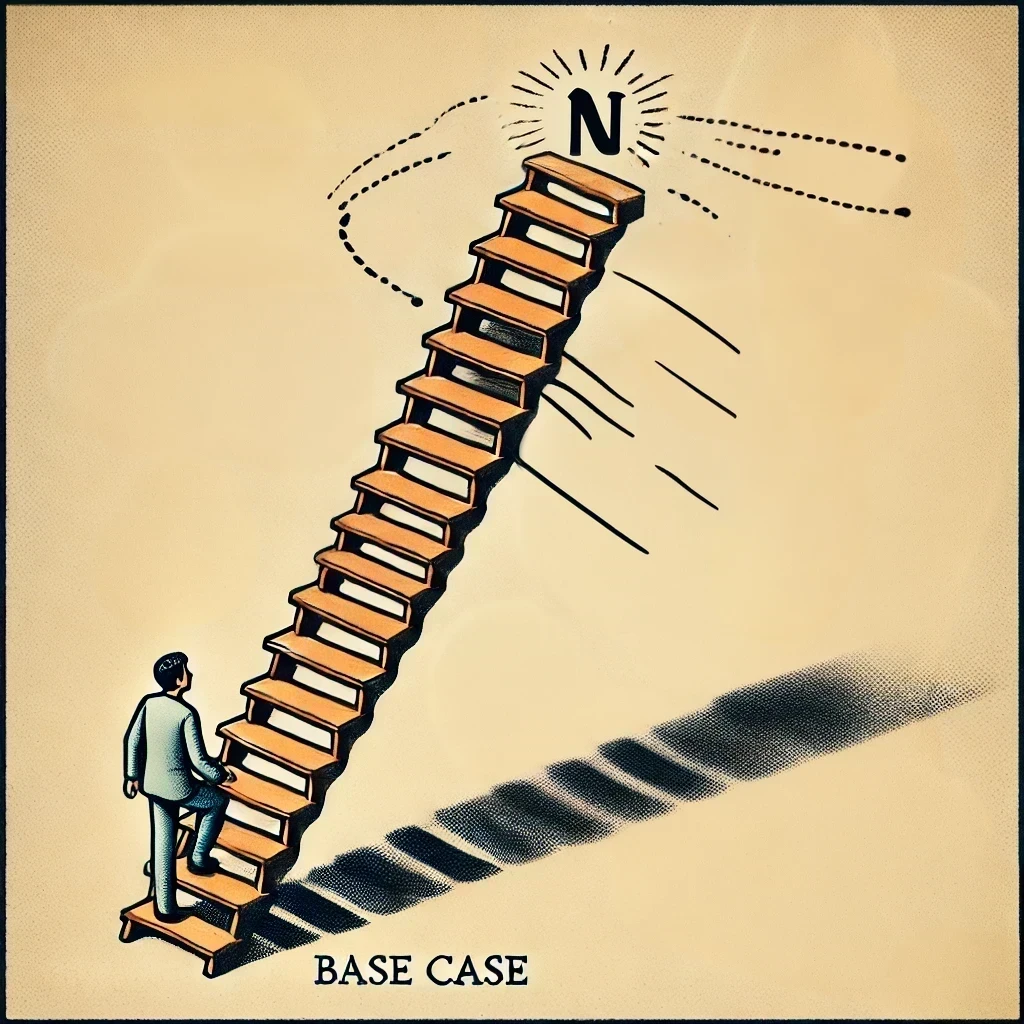
\includegraphics[width=3cm]{images/ladder.png}
    \end{center}
\end{frame}

\subsection{Ejemplo 1. Suma de los primeros \( n \) números enteros positivos}
\begin{frame}{Ejemplo 1. Suma de los primeros \( n \) números enteros positivos}
    \begin{itemize}
        \item Queremos demostrar que: \[ 1 + 2 + 3 + \cdots + n = \frac{n(n+1)}{2} \]
        \item Base de inducción: Para \( n = 1 \):
        \[ 1 = \frac{1(1+1)}{2} = 1 \]
        \item Paso de inducción: Supongamos que la fórmula es cierta para algún \( n = k \), es decir:
        \[ 1 + 2 + 3 + \cdots + k = \frac{k(k+1)}{2} \]
    \end{itemize}
    % Insertar imagen relacionada
\end{frame}

\begin{frame}
    \begin{itemize}
        \item Demostrar que es cierta para \( n = k+1 \):
        \[ 1 + 2 + 3 + \cdots + k + (k+1) = \frac{k(k+1)}{2} + (k+1) \]
        \[ = \frac{k(k+1) + 2(k+1)}{2} = \frac{(k+1)(k+2)}{2} \]
        \item Por lo tanto, la fórmula es verdadera para todo \( n \).
    \end{itemize}
    \begin{center}
        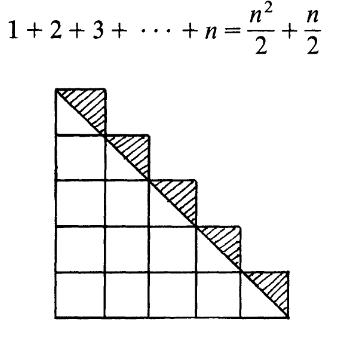
\includegraphics[width=4cm]{images/sum-of-first-n-natural-numbers-proof-3.png}
    \end{center}
\end{frame}

\subsection{Ejemplo 2. La suma de los primeros \( n \) números impares es \( n^2 \)}
\begin{frame}{Ejemplo 2. La suma de los primeros \( n \) números impares es \( n^2 \)}
    \begin{itemize}
        \item Queremos demostrar que: \[ 1 + 3 + 5 + \cdots + (2n-1) = n^2 \]
        \item Base de inducción: Para \( n = 1 \):
        \[ 1 = 1^2 \]
        \item Paso de inducción: Supongamos que la fórmula es cierta para algún \( n = k \), es decir:
        \[ 1 + 3 + 5 + \cdots + (2k-1) = k^2 \]
    \end{itemize}
    % Insertar imagen relacionada
\end{frame}

\begin{frame}
    \begin{itemize}
        \item Demostrar que es cierta para \( n = k+1 \):
        \begin{align*} 1 + 3 + \cdots + (2k-1) + (2(k+1)-1) &= k^2 + 2k+1 \\&= (k+1)^2 \end{align*}
        \item Por lo tanto, la fórmula es verdadera para todo \( n \).
    \end{itemize}
    % Insertar imagen relacionada
\end{frame}
\end{document}